% Options for packages loaded elsewhere
\PassOptionsToPackage{unicode}{hyperref}
\PassOptionsToPackage{hyphens}{url}
\PassOptionsToPackage{dvipsnames,svgnames*,x11names*}{xcolor}
%
\documentclass[
  ignorenonframetext,
]{beamer}
\usepackage{pgfpages}
\setbeamertemplate{caption}[numbered]
\setbeamertemplate{caption label separator}{: }
\setbeamercolor{caption name}{fg=normal text.fg}
\beamertemplatenavigationsymbolsempty
% Prevent slide breaks in the middle of a paragraph
\widowpenalties 1 10000
\raggedbottom
\setbeamertemplate{part page}{
  \centering
  \begin{beamercolorbox}[sep=16pt,center]{part title}
    \usebeamerfont{part title}\insertpart\par
  \end{beamercolorbox}
}
\setbeamertemplate{section page}{
  \centering
  \begin{beamercolorbox}[sep=12pt,center]{part title}
    \usebeamerfont{section title}\insertsection\par
  \end{beamercolorbox}
}
\setbeamertemplate{subsection page}{
  \centering
  \begin{beamercolorbox}[sep=8pt,center]{part title}
    \usebeamerfont{subsection title}\insertsubsection\par
  \end{beamercolorbox}
}
\AtBeginPart{
  \frame{\partpage}
}
\AtBeginSection{
  \ifbibliography
  \else
    \frame{\sectionpage}
  \fi
}
\AtBeginSubsection{
  \frame{\subsectionpage}
}
\usepackage{lmodern}
\usepackage{amssymb,amsmath}
\usepackage{ifxetex,ifluatex}
\ifnum 0\ifxetex 1\fi\ifluatex 1\fi=0 % if pdftex
  \usepackage[T1]{fontenc}
  \usepackage[utf8]{inputenc}
  \usepackage{textcomp} % provide euro and other symbols
\else % if luatex or xetex
  \usepackage{unicode-math}
  \defaultfontfeatures{Scale=MatchLowercase}
  \defaultfontfeatures[\rmfamily]{Ligatures=TeX,Scale=1}
\fi
% Use upquote if available, for straight quotes in verbatim environments
\IfFileExists{upquote.sty}{\usepackage{upquote}}{}
\IfFileExists{microtype.sty}{% use microtype if available
  \usepackage[]{microtype}
  \UseMicrotypeSet[protrusion]{basicmath} % disable protrusion for tt fonts
}{}
\makeatletter
\@ifundefined{KOMAClassName}{% if non-KOMA class
  \IfFileExists{parskip.sty}{%
    \usepackage{parskip}
  }{% else
    \setlength{\parindent}{0pt}
    \setlength{\parskip}{6pt plus 2pt minus 1pt}}
}{% if KOMA class
  \KOMAoptions{parskip=half}}
\makeatother
\usepackage{xcolor}
\IfFileExists{xurl.sty}{\usepackage{xurl}}{} % add URL line breaks if available
\IfFileExists{bookmark.sty}{\usepackage{bookmark}}{\usepackage{hyperref}}
\hypersetup{
  pdftitle={Modeling with Deterministic Functions - Capturing Signal},
  pdfauthor={Zack Treisman},
  colorlinks=true,
  linkcolor=Maroon,
  filecolor=Maroon,
  citecolor=blue,
  urlcolor=Blue,
  pdfcreator={LaTeX via pandoc}}
\urlstyle{same} % disable monospaced font for URLs
\newif\ifbibliography
\usepackage{color}
\usepackage{fancyvrb}
\newcommand{\VerbBar}{|}
\newcommand{\VERB}{\Verb[commandchars=\\\{\}]}
\DefineVerbatimEnvironment{Highlighting}{Verbatim}{commandchars=\\\{\}}
% Add ',fontsize=\small' for more characters per line
\usepackage{framed}
\definecolor{shadecolor}{RGB}{248,248,248}
\newenvironment{Shaded}{\begin{snugshade}}{\end{snugshade}}
\newcommand{\AlertTok}[1]{\textcolor[rgb]{0.94,0.16,0.16}{#1}}
\newcommand{\AnnotationTok}[1]{\textcolor[rgb]{0.56,0.35,0.01}{\textbf{\textit{#1}}}}
\newcommand{\AttributeTok}[1]{\textcolor[rgb]{0.77,0.63,0.00}{#1}}
\newcommand{\BaseNTok}[1]{\textcolor[rgb]{0.00,0.00,0.81}{#1}}
\newcommand{\BuiltInTok}[1]{#1}
\newcommand{\CharTok}[1]{\textcolor[rgb]{0.31,0.60,0.02}{#1}}
\newcommand{\CommentTok}[1]{\textcolor[rgb]{0.56,0.35,0.01}{\textit{#1}}}
\newcommand{\CommentVarTok}[1]{\textcolor[rgb]{0.56,0.35,0.01}{\textbf{\textit{#1}}}}
\newcommand{\ConstantTok}[1]{\textcolor[rgb]{0.00,0.00,0.00}{#1}}
\newcommand{\ControlFlowTok}[1]{\textcolor[rgb]{0.13,0.29,0.53}{\textbf{#1}}}
\newcommand{\DataTypeTok}[1]{\textcolor[rgb]{0.13,0.29,0.53}{#1}}
\newcommand{\DecValTok}[1]{\textcolor[rgb]{0.00,0.00,0.81}{#1}}
\newcommand{\DocumentationTok}[1]{\textcolor[rgb]{0.56,0.35,0.01}{\textbf{\textit{#1}}}}
\newcommand{\ErrorTok}[1]{\textcolor[rgb]{0.64,0.00,0.00}{\textbf{#1}}}
\newcommand{\ExtensionTok}[1]{#1}
\newcommand{\FloatTok}[1]{\textcolor[rgb]{0.00,0.00,0.81}{#1}}
\newcommand{\FunctionTok}[1]{\textcolor[rgb]{0.00,0.00,0.00}{#1}}
\newcommand{\ImportTok}[1]{#1}
\newcommand{\InformationTok}[1]{\textcolor[rgb]{0.56,0.35,0.01}{\textbf{\textit{#1}}}}
\newcommand{\KeywordTok}[1]{\textcolor[rgb]{0.13,0.29,0.53}{\textbf{#1}}}
\newcommand{\NormalTok}[1]{#1}
\newcommand{\OperatorTok}[1]{\textcolor[rgb]{0.81,0.36,0.00}{\textbf{#1}}}
\newcommand{\OtherTok}[1]{\textcolor[rgb]{0.56,0.35,0.01}{#1}}
\newcommand{\PreprocessorTok}[1]{\textcolor[rgb]{0.56,0.35,0.01}{\textit{#1}}}
\newcommand{\RegionMarkerTok}[1]{#1}
\newcommand{\SpecialCharTok}[1]{\textcolor[rgb]{0.00,0.00,0.00}{#1}}
\newcommand{\SpecialStringTok}[1]{\textcolor[rgb]{0.31,0.60,0.02}{#1}}
\newcommand{\StringTok}[1]{\textcolor[rgb]{0.31,0.60,0.02}{#1}}
\newcommand{\VariableTok}[1]{\textcolor[rgb]{0.00,0.00,0.00}{#1}}
\newcommand{\VerbatimStringTok}[1]{\textcolor[rgb]{0.31,0.60,0.02}{#1}}
\newcommand{\WarningTok}[1]{\textcolor[rgb]{0.56,0.35,0.01}{\textbf{\textit{#1}}}}
\usepackage{graphicx,grffile}
\makeatletter
\def\maxwidth{\ifdim\Gin@nat@width>\linewidth\linewidth\else\Gin@nat@width\fi}
\def\maxheight{\ifdim\Gin@nat@height>\textheight\textheight\else\Gin@nat@height\fi}
\makeatother
% Scale images if necessary, so that they will not overflow the page
% margins by default, and it is still possible to overwrite the defaults
% using explicit options in \includegraphics[width, height, ...]{}
\setkeys{Gin}{width=\maxwidth,height=\maxheight,keepaspectratio}
% Set default figure placement to htbp
\makeatletter
\def\fps@figure{htbp}
\makeatother
\setlength{\emergencystretch}{3em} % prevent overfull lines
\providecommand{\tightlist}{%
  \setlength{\itemsep}{0pt}\setlength{\parskip}{0pt}}
\setcounter{secnumdepth}{-\maxdimen} % remove section numbering

\pgfdeclareimage[width=3.5cm]{mcslogo}{../western_logo_hor_MCS_3C_pos.pdf}
\pgfdeclareimage[width=1cm]{ccbysa}{../ccbysa88x31.png}
\titlegraphic{\href{http://creativecommons.org/licenses/by-sa/4.0/}{\pgfuseimage{ccbysa}}
\hfill
\href{https://western.edu/program/mathematics/}{\pgfuseimage{mcslogo}}}
%\usecolortheme{wcu}
%\institute{Western Colorado University}
%\setbeamertemplate{navigation symbols}{}

\title{Modeling with Deterministic Functions - Capturing Signal}
\author{Zack Treisman}
\date{Spring 2021}

\begin{document}
\frame{\titlepage}

\begin{frame}{Philosophy}
\protect\hypertarget{philosophy}{}

Data analysis and statistics are tools used in modeling.

\begin{itemize}
\tightlist
\item
  A \textbf{model} is a proposed distribution of a variable or variables
\item
  Separate any model into two parts: the \textbf{signal} and the
  \textbf{noise}.
\item
  This week we are focused on \textbf{signal}.
\end{itemize}

The most fundamental setting is a pair of variables, \(x\) and \(y\). We
know something about \(x\), and would like to leverage this to learn
something about \(y\), to the extent that this is possible. We call
\(x\) the \textbf{predictor} and \(y\) the \textbf{response}. Write \[
y=f(x)+\epsilon
\] where the model function \(f(x)\) is what we call the \textbf{signal}
and \(\epsilon\) is the \textbf{noise}.

``All models are wrong but some are useful'' - George Box

The usefulness of a model comes when the signal is not drowned out by
the noise. In other words the model is \textbf{statistically
significant}.

\end{frame}

\begin{frame}{xkcd}
\protect\hypertarget{xkcd}{}

\begin{figure}
\centering
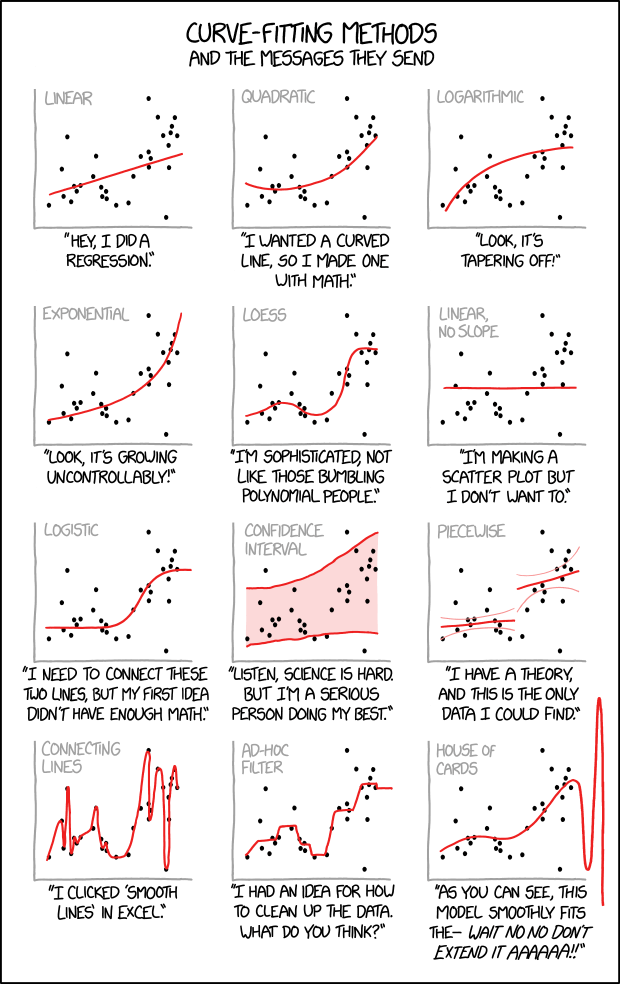
\includegraphics[width=\textwidth,height=0.75\textheight]{curve_fitting.png}
\caption{\url{https://xkcd.com/2048}}
\end{figure}

\end{frame}

\begin{frame}{Model misuse is not a joke}
\protect\hypertarget{model-misuse-is-not-a-joke}{}

\begin{figure}
\centering
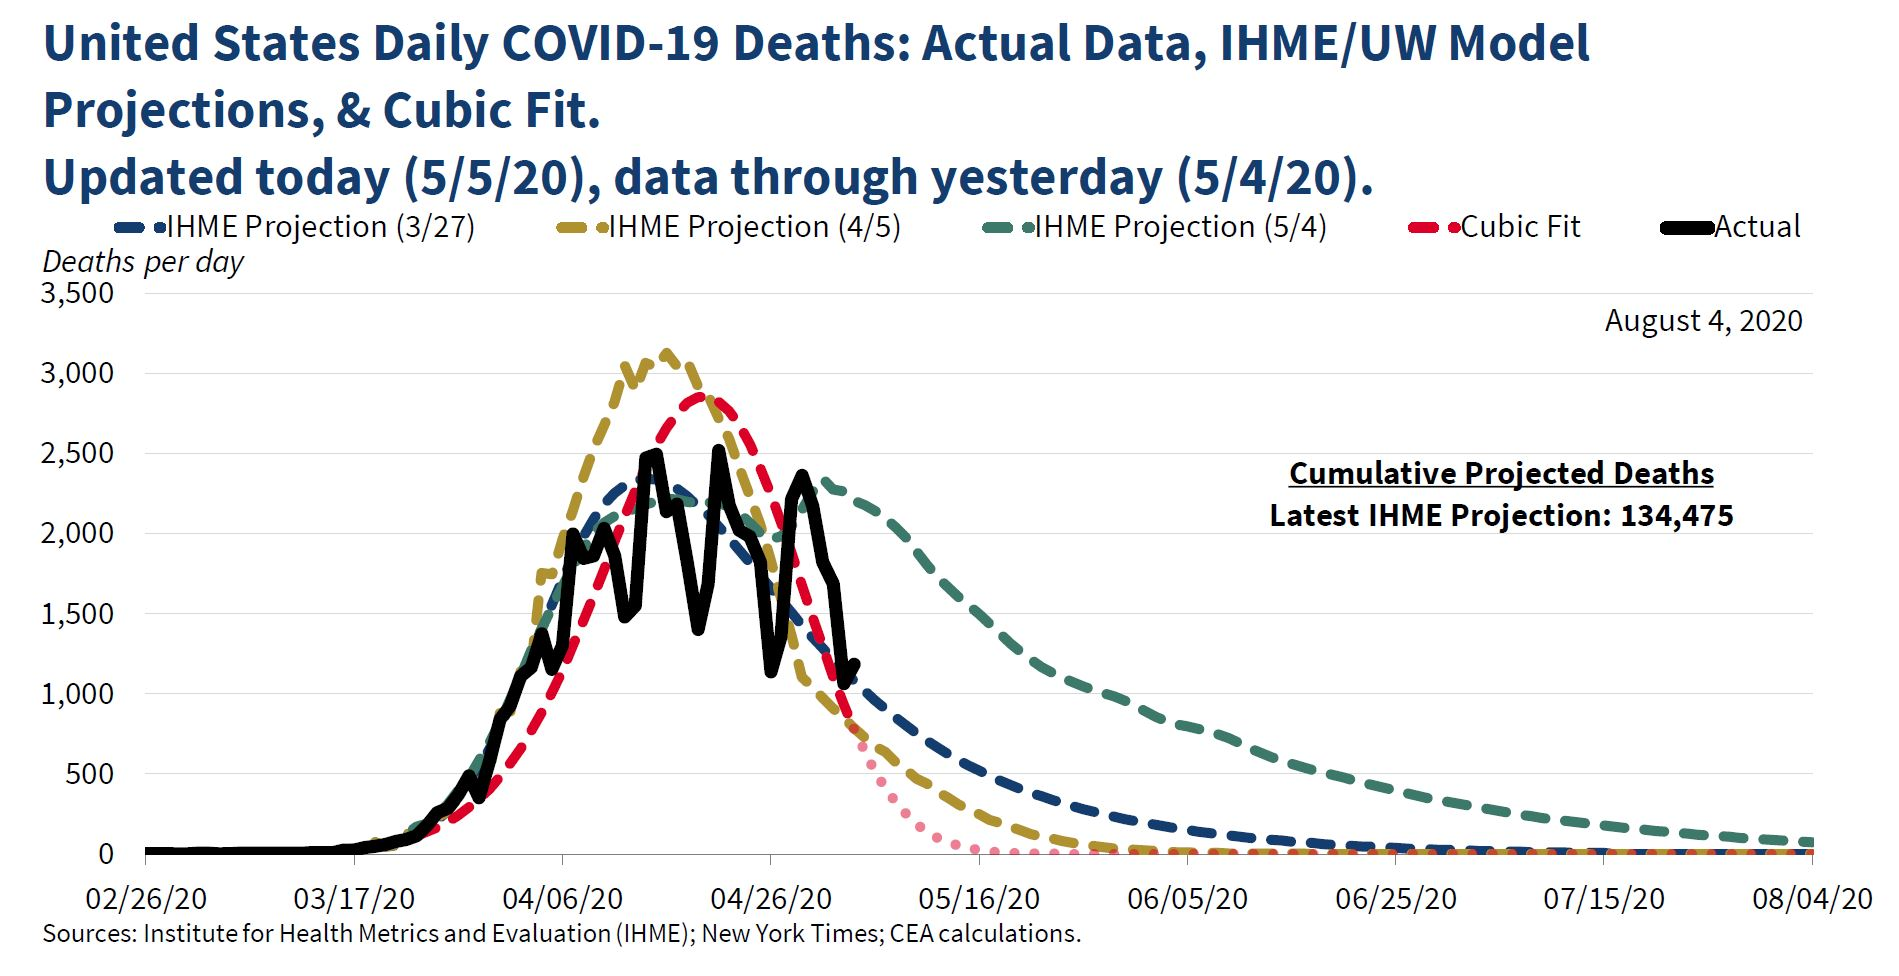
\includegraphics[width=\textwidth,height=0.75\textheight]{covid.jpeg}
\caption{\url{https://twitter.com/WhiteHouseCEA/status/1257680258364555264}}
\end{figure}

\end{frame}

\begin{frame}{Reducible and irreducible error}
\protect\hypertarget{reducible-and-irreducible-error}{}

If we had infinite knowledge, we could choose for our model function the
expected value, or mean, of all \(y\) such that \((x,y)\) is a possible
data point. Write \(\mu(x)\) for this expected value. \[
y=\mu(x)+\varepsilon
\] We call \(\varepsilon\) the \textbf{irreducible error} or
\textbf{intrinsic variance}. It is the uncertainty that exists because
of natural variation in the system described.

Any actual model function that we come up with will differ from this
optimal function. Suppose we have a model function \(f(x)\). We call the
difference \(f(x)-\mu(x)\) the \textbf{reducible error}. With a better
\(f\) we can reduce the reducible error.

\end{frame}

\begin{frame}{Bias and Variance}
\protect\hypertarget{bias-and-variance}{}

The reducible error can be broken down into two parts.

\begin{itemize}
\tightlist
\item
  The error due to \textbf{bias} is that part of the reducible error
  that comes from a model function's inability to change when it needs
  to.
\item
  The error due to \textbf{variance} is that part of the reducible error
  that comes from a model function's excessive flexibility to match the
  particular data that are observed.
\end{itemize}

A model function with high bias error is said to \textbf{underfit} the
data, and one with high variance error is an \textbf{overfit}. Whenever
we are choosing a model, we must consider this \textbf{bias-variance
tradeoff}.

\end{frame}

\begin{frame}{Parametric vs Non-parametric models}
\protect\hypertarget{parametric-vs-non-parametric-models}{}

\begin{itemize}
\tightlist
\item
  A \textbf{parametric} model function is one defined in terms of
  arithmetic and analytic functions, such as logarithms, polynomials, or
  anything else you might have encountered in a math class like
  Calculus. The numbers such as coefficients and exponents defining the
  function are called the \textbf{parameters}.
\item
  A \textbf{non-parametric} model function is defined in some other way.
  The first example we will encounter and use is \emph{local regression}
  or \emph{loess}. Trees and random forests are also non-parametric
  models.
\end{itemize}

\end{frame}

\begin{frame}[fragile]{Linear function models}
\protect\hypertarget{linear-function-models}{}

If \(x\) and \(y\) are both numeric variables, then the simplest
possible relationship between them is a linear relationship. \[
y = \beta_0 + \beta_1 x +\epsilon
\]

\begin{itemize}
\tightlist
\item
  \(\beta_0\) is the \emph{intercept}, the value we predict for \(y\)
  when \(x\) is zero.
\item
  \(\beta_1\) is the \emph{slope}, or predicted rate of change in \(y\)
  with respect to \(x\). Often written \(\frac{\Delta y}{\Delta x}\) or
  \(\frac{dy}{dx}\).
\end{itemize}

The tremendous advantage of the linear function model over all others is
its simplicity. A disadvantage is a tendency towards high bias error.

Note: This model is linear in the variable \(x\) \textbf{and} in the
\emph{parameters} \(\beta_i\). The term ``linear model'' is frequently
applied with both meanings, but the latter is more useful. The R command
\texttt{lm} refers to linearity in the parameters.

\end{frame}

\begin{frame}{Linear models with multiple predictors}
\protect\hypertarget{linear-models-with-multiple-predictors}{}

Extending to multiple predictor variables is straightforward. \[
y=\beta_0 + \beta_1 x_1 +\beta_2 x_2 +\beta_3 x_3 + \epsilon
\]

\begin{itemize}
\tightlist
\item
  \(\beta_i\) is the expected change in \(y\) as \(x_i\) changes and all
  else is constant.
\item
  If the \(x_i\) are correlated, these models can be unreliable.
\end{itemize}

\end{frame}

\begin{frame}{Linear models with categorical predictors}
\protect\hypertarget{linear-models-with-categorical-predictors}{}

If a predictor variable is categorical, the linear model can still be
used.

\begin{itemize}
\tightlist
\item
  One level is set as the \textbf{reference} level of the variable.
\item
  For every other level of the variable, an \textbf{indicator variable}
  is defined, taking the value 1 when the variable has that level and 0
  otherwise.
\item
  The coefficient \(\beta_i\) is the expected effect from observing
  level \(i\) instead of the reference level.
\end{itemize}

Examples:

\begin{itemize}
\tightlist
\item
  Control/ Treatment: Control is reference, \(x_\text{treat}\)
\item
  Low/ Medium/ High: Low is reference, \(x_\text{med}, x_\text{high}\)
\end{itemize}

\end{frame}

\begin{frame}[fragile]{Polynomial functions}
\protect\hypertarget{polynomial-functions}{}

Including powers of \(x\) such as \(x^2\) or \(x^3\) can reduce bias.

Example: \[
y=\beta_0+\beta_1 x + \beta_2 x^2 +\epsilon
\] This is still a linear model even though it includes the \(x^2\)
term.

\scriptsize

\begin{Shaded}
\begin{Highlighting}[]
\KeywordTok{ggplot}\NormalTok{(mtcars, }\KeywordTok{aes}\NormalTok{(mpg, hp)) }\OperatorTok{+}\StringTok{ }\KeywordTok{geom_point}\NormalTok{(}\DataTypeTok{alpha=}\FloatTok{0.5}\NormalTok{) }\OperatorTok{+}
\StringTok{  }\KeywordTok{geom_smooth}\NormalTok{(}\DataTypeTok{method =}\NormalTok{ lm, }\DataTypeTok{formula =}\NormalTok{ y}\OperatorTok{~}\NormalTok{x, }\DataTypeTok{se=}\NormalTok{F) }\OperatorTok{+}
\StringTok{  }\KeywordTok{geom_smooth}\NormalTok{(}\DataTypeTok{method =}\NormalTok{ lm, }\DataTypeTok{formula =}\NormalTok{ y}\OperatorTok{~}\KeywordTok{poly}\NormalTok{(x,}\DecValTok{2}\NormalTok{), }\DataTypeTok{se=}\NormalTok{F, }\DataTypeTok{color=}\StringTok{"red"}\NormalTok{)}
\end{Highlighting}
\end{Shaded}

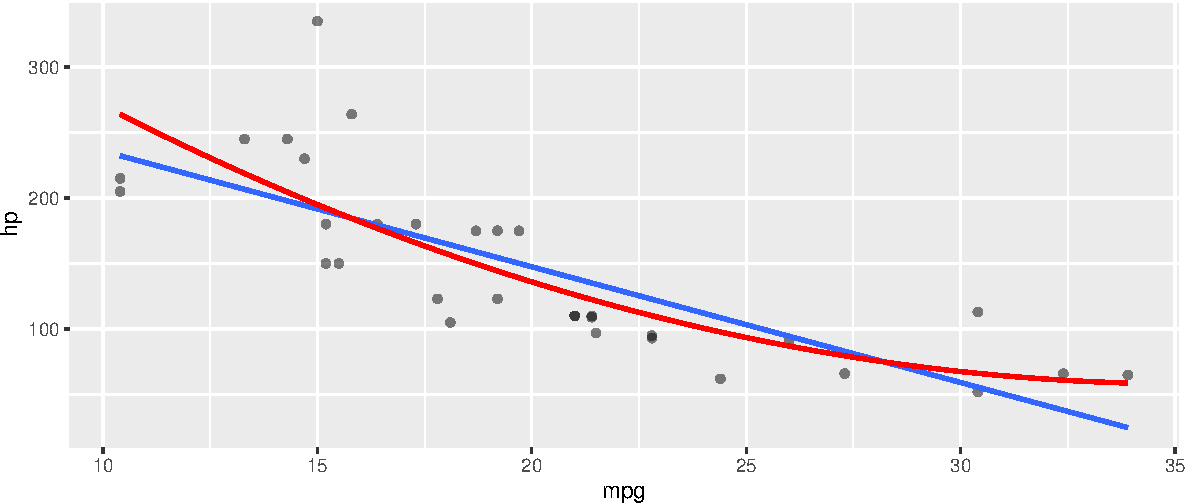
\includegraphics{signal_files/figure-beamer/unnamed-chunk-2-1.pdf}

\end{frame}

\begin{frame}{Power functions}
\protect\hypertarget{power-functions}{}

A power function model is of the form \[
y=a x^k + \epsilon
\] Note that \(k\) can be any number, not just a positive integer. This
is \emph{not} a linear model because of the parameter \(k\).

\begin{itemize}
\tightlist
\item
  Power models can have explanatory meaning if \(x\) and \(y\) have
  relevant dimensionality, like mass or area.
\end{itemize}

Power function models can be fit using linear model techniques by taking
logarithms. Ignoring the error term for a moment: \[
\hat{y}=a x^k \qquad \iff \qquad \log(\hat{y})=\log(a)+k\log(x)
\]

\end{frame}

\begin{frame}{Back-transforms and error}
\protect\hypertarget{back-transforms-and-error}{}

Models fit on log-transformed variables can be exponentiated back to the
original variables. How the error transforms can cause issues.

\begin{itemize}
\tightlist
\item
  Exponentiating the predicted mean of a log-transformed variable does
  \textbf{not} predict the untransformed mean.

  \begin{itemize}
  \tightlist
  \item
    When back-transforming, add half the variance in the residuals
    before exponentiating to recover the mean.
  \item
    Diagnostics such as \(R^2\) and p values apply to the transformed
    variables, not after back-transformation.
  \end{itemize}
\item
  Linear regression assumes that the error is additive. Exponentiation
  changes this addition into multiplication.
\end{itemize}

Suppose we fit a model: \[
\log(y)\sim N\left(\hat\beta_0+\hat\beta_1\log(x), \sigma^2\right).
\] Then the prediction for the mean of \(y\) is \[
e^{\hat\beta_0+\hat\beta_1\log(x)+\sigma^2/2}=e^{\hat\beta_0+\sigma^2/2}x^{\hat\beta_1}
\] and the variance is dependent on \(x\).

\end{frame}

\begin{frame}[fragile]{\href{https://en.wikipedia.org/wiki/Kleiber\%27s_law}{Kleiber's
law}}
\protect\hypertarget{kleibers-law}{}

Mass and metabolic rate of mammals relate via a power law. \scriptsize

\begin{Shaded}
\begin{Highlighting}[]
\KeywordTok{ggplot}\NormalTok{(ex0826, }\KeywordTok{aes}\NormalTok{(Mass, Metab)) }\OperatorTok{+}\StringTok{ }\KeywordTok{geom_point}\NormalTok{() }\OperatorTok{+}\StringTok{ }\CommentTok{# data in Sleuth3}
\StringTok{  }\KeywordTok{scale_x_log10}\NormalTok{() }\OperatorTok{+}\StringTok{ }\KeywordTok{scale_y_log10}\NormalTok{() }\OperatorTok{+}\StringTok{ }\KeywordTok{geom_smooth}\NormalTok{(}\DataTypeTok{method =}\NormalTok{ lm, }\DataTypeTok{se=}\NormalTok{F)}
\end{Highlighting}
\end{Shaded}

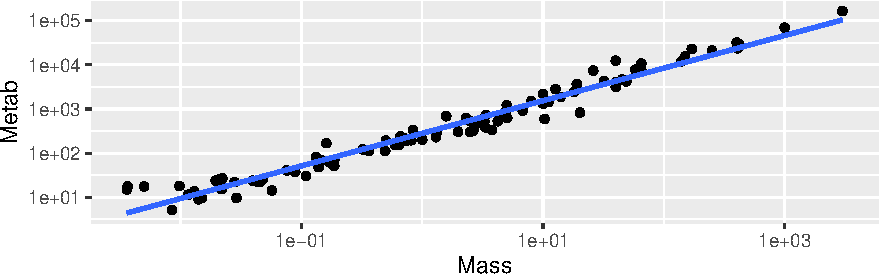
\includegraphics{signal_files/figure-beamer/unnamed-chunk-3-1.pdf}

\begin{Shaded}
\begin{Highlighting}[]
\NormalTok{lm1 <-}\StringTok{ }\KeywordTok{lm}\NormalTok{(}\KeywordTok{log}\NormalTok{(Metab)}\OperatorTok{~}\KeywordTok{log}\NormalTok{(Mass), }\DataTypeTok{data =}\NormalTok{ ex0826)}
\NormalTok{lm1}\OperatorTok{$}\NormalTok{coefficients; }\KeywordTok{var}\NormalTok{(lm1}\OperatorTok{$}\NormalTok{residuals)}
\end{Highlighting}
\end{Shaded}

\begin{verbatim}
## (Intercept)   log(Mass) 
##   5.6383307   0.7387436
\end{verbatim}

\begin{verbatim}
## [1] 0.2068395
\end{verbatim}

\normalsize

\[
\text{Metab}=e^{5.64+0.21/2}\times(\text{Mass})^{\only<2->{\alert}{0.74}} \times \epsilon
\]

\end{frame}

\begin{frame}[fragile]{Rational models}
\protect\hypertarget{rational-models}{}

The ratio of two polynomials is called a \textbf{rational function}.
They can have asymptotes. Not generally linearizable.

Example: Michaelis-Menten/ Holling (McNickle and Brown (2014)) \[
f(x)=\frac{ax}{b+x}
\] \scriptsize

\begin{Shaded}
\begin{Highlighting}[]
\KeywordTok{curve}\NormalTok{(}\DecValTok{3}\OperatorTok{*}\NormalTok{x}\OperatorTok{/}\NormalTok{(}\DecValTok{5}\OperatorTok{+}\NormalTok{x), }\DataTypeTok{from =} \DecValTok{0}\NormalTok{, }\DataTypeTok{to =} \DecValTok{50}\NormalTok{, }\DataTypeTok{ylim =} \KeywordTok{c}\NormalTok{(}\DecValTok{0}\NormalTok{, }\DecValTok{4}\NormalTok{), }\DataTypeTok{ylab =} \StringTok{"y"}\NormalTok{)}
\KeywordTok{abline}\NormalTok{(}\DataTypeTok{h=}\DecValTok{3}\NormalTok{, }\DataTypeTok{lty =} \DecValTok{4}\NormalTok{); }\KeywordTok{abline}\NormalTok{(}\DecValTok{0}\NormalTok{, }\DecValTok{3}\OperatorTok{/}\DecValTok{5}\NormalTok{, }\DataTypeTok{lty =} \DecValTok{2}\NormalTok{)}
\KeywordTok{text}\NormalTok{(}\DecValTok{5}\NormalTok{, }\FloatTok{0.3}\NormalTok{, }\StringTok{"slope a/b at 0"}\NormalTok{); }\KeywordTok{text}\NormalTok{(}\DecValTok{40}\NormalTok{, }\FloatTok{3.3}\NormalTok{, }\StringTok{"asymptote at y=a"}\NormalTok{) }
\end{Highlighting}
\end{Shaded}

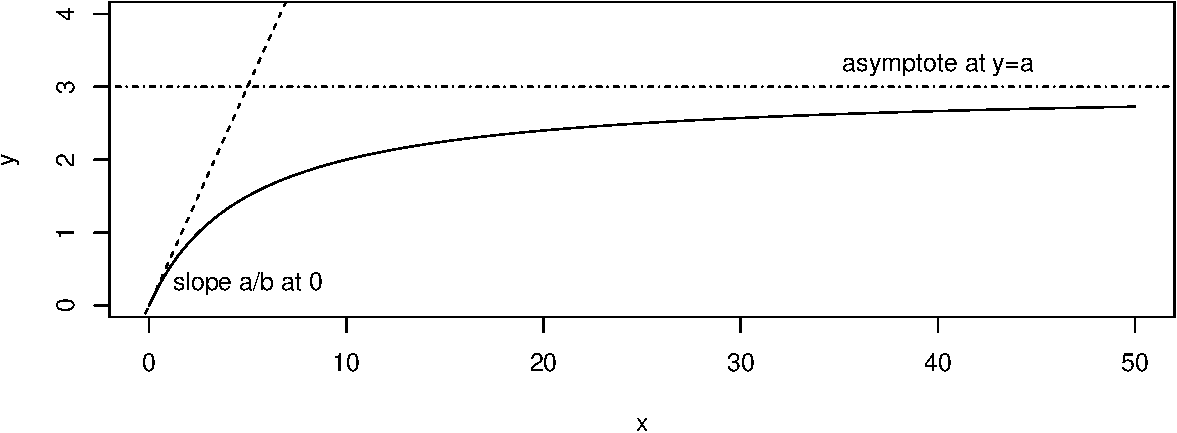
\includegraphics{signal_files/figure-beamer/unnamed-chunk-4-1.pdf}

\end{frame}

\begin{frame}{Exponential models}
\protect\hypertarget{exponential-models}{}

Exponential growth and decay are very common.

\begin{itemize}
\tightlist
\item
  \(\frac{dy}{dx}\) means change in \(y\) as \(x\) changes.
\item
  \(\frac{dy}{dx}=k \cdot y\) means \(y\) changes by a fixed fraction
  (\(k\)) of itself.
\end{itemize}

The solution is \[
y=a\,e^{kx}+\epsilon
\]

Growth if \(k>0\), decline if \(k<0\).

\begin{itemize}
\tightlist
\item
  Exponential growth is usually bad for extrapolation. Something else
  tends to take over.
\item
  With a little algebra, exponential decay can be used to model
  convergence to any asymptote.
\end{itemize}

These models are not linear, but taking logs make them so: \[
\hat{y}=a\,e^{kx} \qquad \iff \qquad \log(\hat{y})=\log(a)+kx
\]

\end{frame}

\begin{frame}[fragile]{Exponential decay example}
\protect\hypertarget{exponential-decay-example}{}

Exponential decay has long been used to model decomposition of biotic
material. Olson (1963)

\scriptsize

\begin{Shaded}
\begin{Highlighting}[]
\CommentTok{# Simulated data, see RMarkdown for code.}
\KeywordTok{ggplot}\NormalTok{(decay, }\KeywordTok{aes}\NormalTok{(age, mass, }\DataTypeTok{color=}\NormalTok{species))}\OperatorTok{+}\StringTok{  }
\StringTok{  }\KeywordTok{expand_limits}\NormalTok{(}\DataTypeTok{y=}\DecValTok{0}\NormalTok{)}\OperatorTok{+}
\StringTok{  }\KeywordTok{geom_point}\NormalTok{()}\OperatorTok{+}
\StringTok{  }\KeywordTok{geom_smooth}\NormalTok{(}\DataTypeTok{method=}\StringTok{"glm"}\NormalTok{, }
              \DataTypeTok{method.args =} \KeywordTok{list}\NormalTok{(}\DataTypeTok{family=}\KeywordTok{gaussian}\NormalTok{(}\DataTypeTok{link=}\StringTok{"log"}\NormalTok{)),}
              \DataTypeTok{se=}\OtherTok{FALSE}\NormalTok{)}
\end{Highlighting}
\end{Shaded}

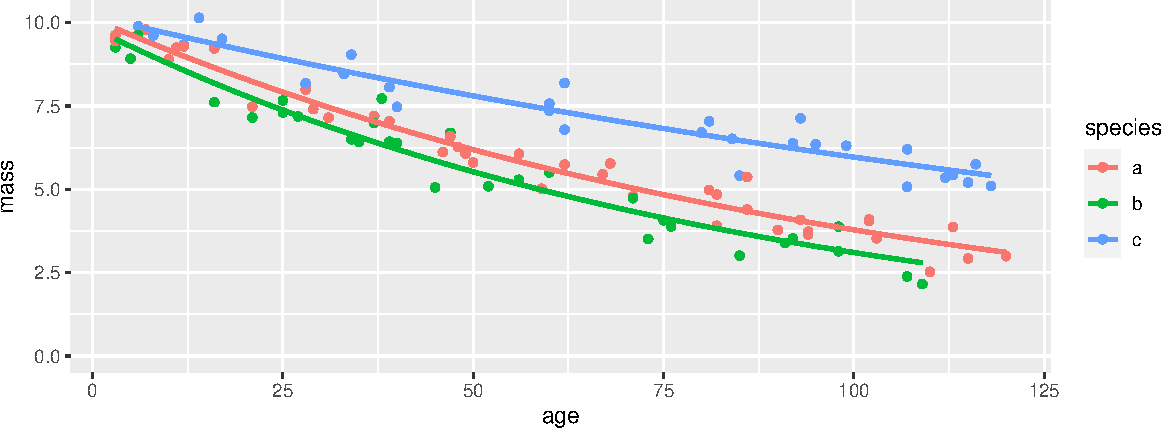
\includegraphics{signal_files/figure-beamer/unnamed-chunk-6-1.pdf}

\end{frame}

\begin{frame}[fragile]{Decay model using log-transformed \texttt{mass}}
\protect\hypertarget{decay-model-using-log-transformed-mass}{}

In this model \texttt{speciesb} and \texttt{speciesc} are not
significant at \(\alpha=0.05\) but the interaction terms are, so their
initial quantities do not appear to differ from species a, but their
decay rates do.

\scriptsize

\begin{Shaded}
\begin{Highlighting}[]
\NormalTok{lm2 <-}\StringTok{ }\KeywordTok{lm}\NormalTok{(}\KeywordTok{log}\NormalTok{(mass)}\OperatorTok{~}\NormalTok{age}\OperatorTok{*}\NormalTok{species, }\DataTypeTok{data=}\NormalTok{decay)}
\KeywordTok{round}\NormalTok{(}\KeywordTok{summary}\NormalTok{(lm2)}\OperatorTok{$}\NormalTok{coefficients,}\DecValTok{4}\NormalTok{)}
\end{Highlighting}
\end{Shaded}

\begin{verbatim}
##              Estimate Std. Error  t value Pr(>|t|)
## (Intercept)    2.3225     0.0283  81.9712   0.0000
## age           -0.0100     0.0004 -24.5589   0.0000
## speciesb      -0.0059     0.0434  -0.1363   0.8919
## speciesc       0.0019     0.0455   0.0410   0.9674
## age:speciesb  -0.0023     0.0007  -3.3980   0.0010
## age:speciesc   0.0046     0.0006   7.5162   0.0000
\end{verbatim}

\begin{Shaded}
\begin{Highlighting}[]
\KeywordTok{round}\NormalTok{(}\KeywordTok{var}\NormalTok{(lm2}\OperatorTok{$}\NormalTok{residuals),}\DecValTok{4}\NormalTok{)}
\end{Highlighting}
\end{Shaded}

\begin{verbatim}
## [1] 0.008
\end{verbatim}

\normalsize

The model for the mean is: \[
\text{mass} = 10.242 \times e^{(-0.01-0.0023\chi_b+0.0046\chi_c)\text{age}}\times\epsilon
\] \(10.242 = e^{2.3225+0.008/2}\) and \(\chi_b\) and \(\chi_c\) are
indicator functions.

\end{frame}

\begin{frame}{Link functions}
\protect\hypertarget{link-functions}{}

Most people who fit models to log transformed variables don't do the
back-transformation. But this means that they aren't actually talking
about the variables in the system they want to model.

\textbf{Generalized linear models} (GLMs) offer a solution: link
functions. The mathematics of computing the parameters is more
complicated, but they give a model that for untransformed variables.

A GLM with a log link for \(y\) in terms of \(x\) fits: \[
\log(\mu_y)=\beta_0+\beta_1x
\] or equivalently \[
\mu_y=e^{\beta_0+\beta_1x}
\] and the error is homoscedastic, as we like it.

Using GLMs and link functions means we can talk about our variables, not
their transforms.

\end{frame}

\begin{frame}[fragile]{Decay model using \texttt{glm} and log link}
\protect\hypertarget{decay-model-using-glm-and-log-link}{}

Specifying a link function for a GLM in R is done in the \texttt{family}
argument, which is used to describe the shape of the error. For normally
distributed error, use \texttt{family=gaussian}.

\scriptsize

\begin{Shaded}
\begin{Highlighting}[]
\NormalTok{lm2a <-}\StringTok{ }\KeywordTok{glm}\NormalTok{(mass}\OperatorTok{~}\NormalTok{age}\OperatorTok{*}\NormalTok{species, }\DataTypeTok{family=}\KeywordTok{gaussian}\NormalTok{(}\DataTypeTok{link=}\NormalTok{log), }\DataTypeTok{data=}\NormalTok{decay)}
\KeywordTok{round}\NormalTok{(}\KeywordTok{summary}\NormalTok{(lm2a)}\OperatorTok{$}\NormalTok{coefficients, }\DecValTok{4}\NormalTok{)}
\end{Highlighting}
\end{Shaded}

\begin{verbatim}
##              Estimate Std. Error  t value Pr(>|t|)
## (Intercept)    2.3150     0.0185 125.4186   0.0000
## age           -0.0098     0.0004 -25.8990   0.0000
## speciesb      -0.0280     0.0300  -0.9342   0.3526
## speciesc       0.0082     0.0278   0.2947   0.7689
## age:speciesb  -0.0017     0.0007  -2.5257   0.0132
## age:speciesc   0.0045     0.0005   8.9756   0.0000
\end{verbatim}

\normalsize

Note the increase in the p-value for the \texttt{age:speciesb} term.

\begin{itemize}
\tightlist
\item
  It is possible that a difference between groups can appear significant
  for log transformed variables but not when we look at the variables
  directly.
\end{itemize}

\end{frame}

\begin{frame}[fragile]{Logistic models}
\protect\hypertarget{logistic-models}{}

The logistic function makes a transition from \(y=0\) to \(y=1\). \[
y=\frac{e^{a+bx}}{1+e^{a+bx}}
\]

\scriptsize

\begin{Shaded}
\begin{Highlighting}[]
\KeywordTok{curve}\NormalTok{(}\KeywordTok{exp}\NormalTok{(}\OperatorTok{-}\DecValTok{7}\OperatorTok{+}\DecValTok{3}\OperatorTok{*}\NormalTok{x)}\OperatorTok{/}\NormalTok{(}\DecValTok{1}\OperatorTok{+}\KeywordTok{exp}\NormalTok{(}\OperatorTok{-}\DecValTok{7}\OperatorTok{+}\DecValTok{3}\OperatorTok{*}\NormalTok{x)), }\DataTypeTok{from=}\DecValTok{0}\NormalTok{, }\DataTypeTok{to=}\DecValTok{4}\NormalTok{, }\DataTypeTok{ylim=}\KeywordTok{c}\NormalTok{(}\DecValTok{0}\NormalTok{, }\DecValTok{1}\NormalTok{), }\DataTypeTok{ylab=}\StringTok{"y"}\NormalTok{)}
\end{Highlighting}
\end{Shaded}

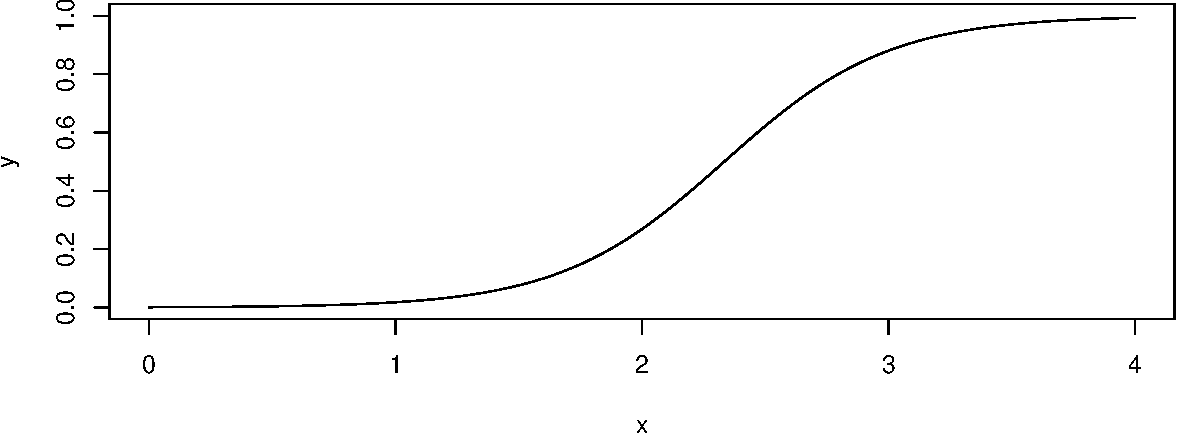
\includegraphics{signal_files/figure-beamer/unnamed-chunk-9-1.pdf}

\normalsize

\begin{itemize}
\tightlist
\item
  Mostly used for binary classification. (logistic regression)
\item
  Also useful for populations with a carrying capacity.
\end{itemize}

Model with \texttt{link=logit} in \texttt{glm}. Default for
\texttt{family=binomial}.

\end{frame}

\begin{frame}{Piecewise models}
\protect\hypertarget{piecewise-models}{}

Bolker (2008) Figure 3.7.

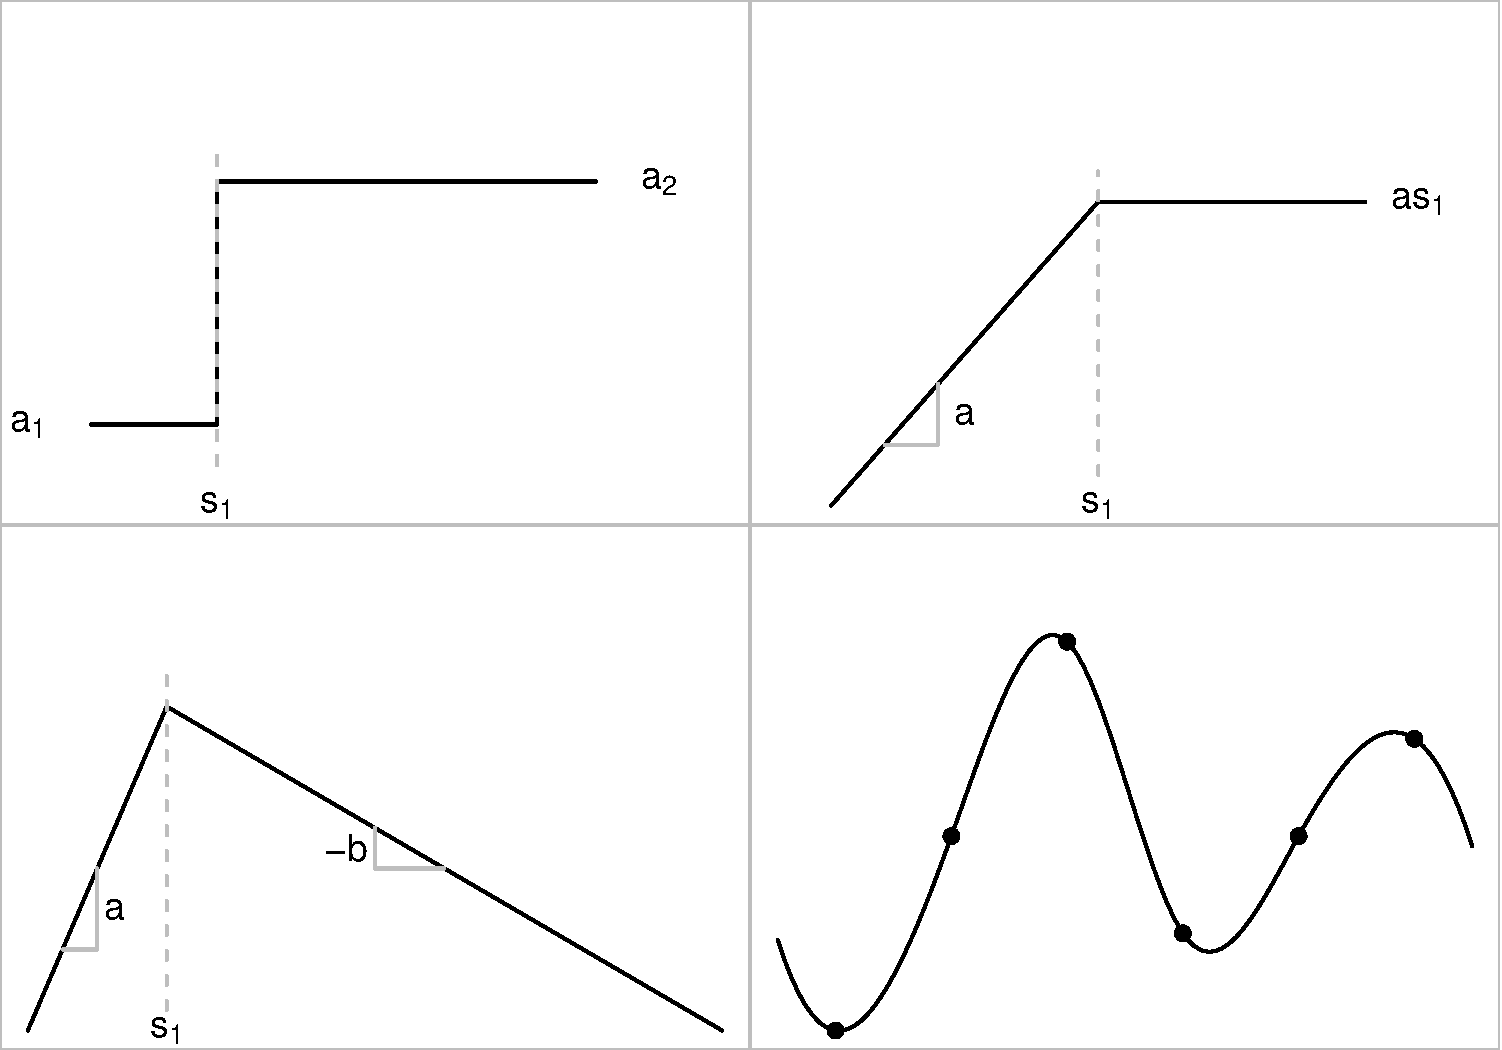
\includegraphics{signal_files/figure-beamer/unnamed-chunk-10-1.pdf}

\end{frame}

\begin{frame}[fragile]{Splines}
\protect\hypertarget{splines}{}

Weather drives the response. A spline can help account for this.

\scriptsize

\begin{Shaded}
\begin{Highlighting}[]
\NormalTok{SoilMoist <-}\StringTok{ }\KeywordTok{read.csv}\NormalTok{(}\StringTok{"data/SoilMoisture_ALL.csv"}\NormalTok{) }\CommentTok{# Alexia Cooper's data}
\NormalTok{SoilMoist}\OperatorTok{$}\NormalTok{TimeStamp <-}\StringTok{ }\KeywordTok{mdy}\NormalTok{(SoilMoist}\OperatorTok{$}\NormalTok{TimeStamp)}
\NormalTok{splinemod <-}\StringTok{ }\KeywordTok{lm}\NormalTok{(Moisture}\OperatorTok{~}\KeywordTok{ns}\NormalTok{(TimeStamp,}\DecValTok{4}\NormalTok{), }\DataTypeTok{data=}\NormalTok{SoilMoist)}
\NormalTok{SoilMoist}\OperatorTok{$}\NormalTok{pred <-}\StringTok{ }\KeywordTok{predict}\NormalTok{(splinemod)}
\KeywordTok{ggplot}\NormalTok{(SoilMoist, }\KeywordTok{aes}\NormalTok{(TimeStamp,Moisture, }\DataTypeTok{color =}\NormalTok{ Treat))}\OperatorTok{+}
\StringTok{  }\KeywordTok{facet_wrap}\NormalTok{(}\OperatorTok{~}\NormalTok{Site)}\OperatorTok{+}\KeywordTok{geom_point}\NormalTok{()}\OperatorTok{+}\KeywordTok{geom_line}\NormalTok{(}\KeywordTok{aes}\NormalTok{(}\DataTypeTok{y=}\NormalTok{pred))}
\end{Highlighting}
\end{Shaded}

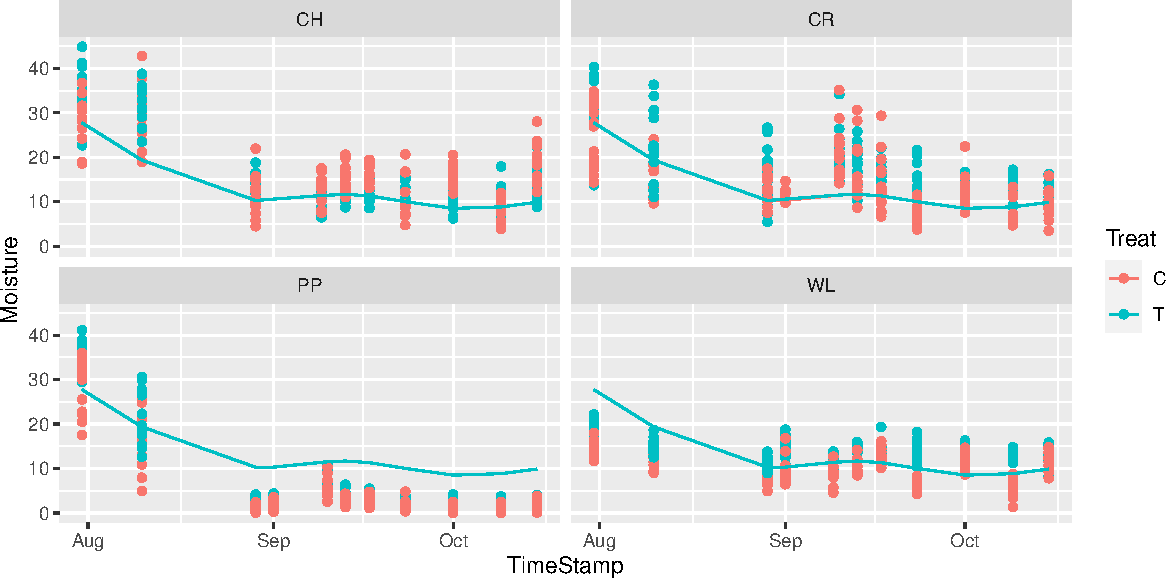
\includegraphics{signal_files/figure-beamer/unnamed-chunk-11-1.pdf}

\end{frame}

\begin{frame}{Nearest neighbor averaging (knn)}
\protect\hypertarget{nearest-neighbor-averaging-knn}{}

\begin{itemize}
\tightlist
\item
  Assume the actual expected value function doesn't change too quickly:
  \(\mu(x-h)\approx\mu(x)\approx\mu(x+h)\).
\end{itemize}

Choose a positive integer \(k\) and define \(f(x)\) as the average of
\(y_i\) for the points \((x_i,y_i)\) where \(x-x_i\) is among the \(k\)
smallest.

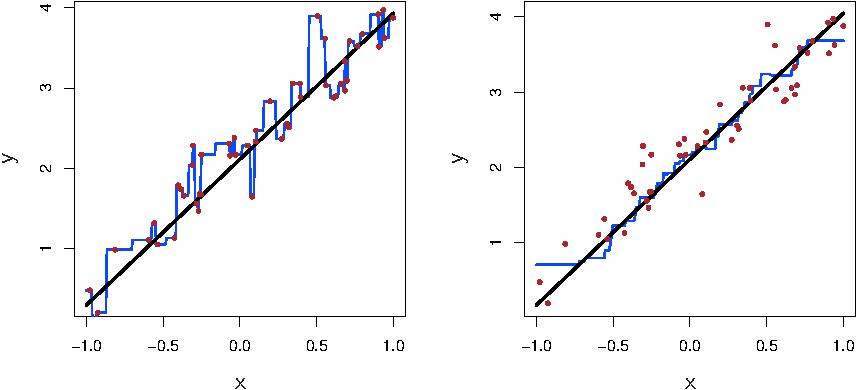
\includegraphics{../images/knn2.pdf}

Left: knn with \(k=1\). Variance is high. Right: knn with \(k=9\).

\end{frame}

\begin{frame}{Weighted averaging and local regression (loess)}
\protect\hypertarget{weighted-averaging-and-local-regression-loess}{}

Choose a distance and define \(f(x)\) by linear regression using the
data within that distance of \(x\) or weighted based on that distance.

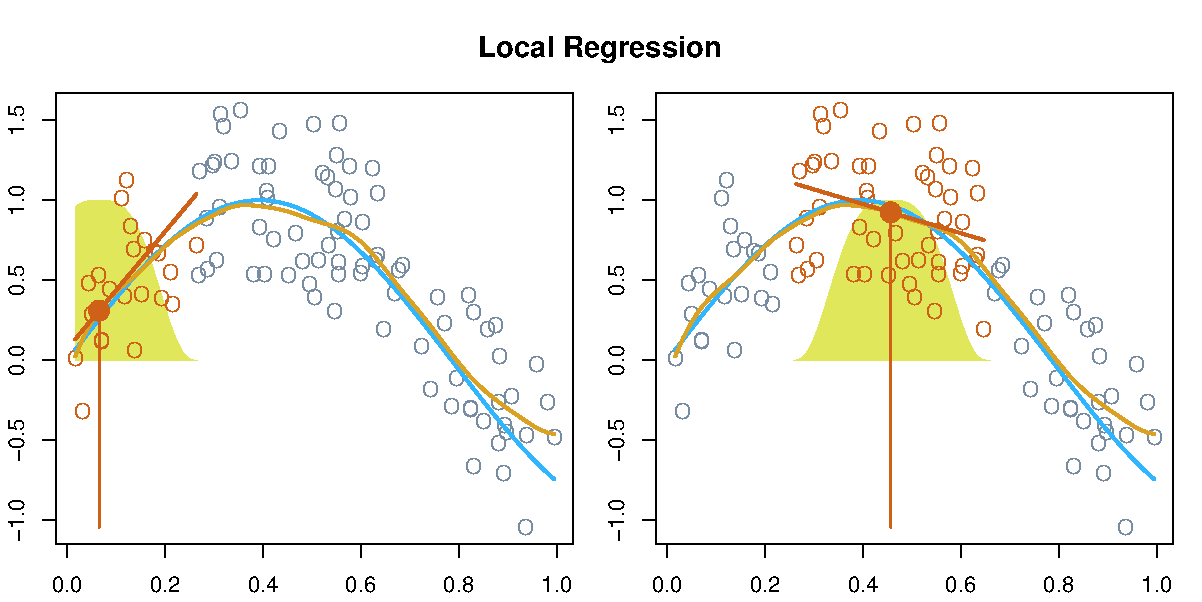
\includegraphics{../images/loess.pdf}

Simulated data. Blue curve is the true signal, orange is the weighted
local regression.

\end{frame}

\begin{frame}[fragile]{Loess in R}
\protect\hypertarget{loess-in-r}{}

One way to do loess in R is to use \texttt{gam} and \texttt{lo}.

\scriptsize

\begin{Shaded}
\begin{Highlighting}[]
\NormalTok{moistmod0 <-}\StringTok{ }\KeywordTok{gam}\NormalTok{(Moisture}\OperatorTok{~}\KeywordTok{lo}\NormalTok{(TimeStamp), }\DataTypeTok{data=}\NormalTok{SoilMoist)}
\NormalTok{moistmod1 <-}\StringTok{ }\KeywordTok{gam}\NormalTok{(Moisture}\OperatorTok{~}\KeywordTok{lo}\NormalTok{(TimeStamp)}\OperatorTok{+}\NormalTok{Site, }\DataTypeTok{data=}\NormalTok{SoilMoist)}
\NormalTok{moistmod2 <-}\StringTok{ }\KeywordTok{gam}\NormalTok{(Moisture}\OperatorTok{~}\KeywordTok{lo}\NormalTok{(TimeStamp)}\OperatorTok{+}\NormalTok{Site}\OperatorTok{+}\NormalTok{Treat, }\DataTypeTok{data=}\NormalTok{SoilMoist)}
\NormalTok{moistmod3 <-}\StringTok{ }\KeywordTok{gam}\NormalTok{(Moisture}\OperatorTok{~}\KeywordTok{lo}\NormalTok{(TimeStamp)}\OperatorTok{+}\NormalTok{Site}\OperatorTok{*}\NormalTok{Treat, }\DataTypeTok{data=}\NormalTok{SoilMoist)}
\KeywordTok{anova}\NormalTok{(moistmod0, moistmod1, moistmod2, moistmod3, }\DataTypeTok{test=}\StringTok{"F"}\NormalTok{)}
\end{Highlighting}
\end{Shaded}

\begin{verbatim}
## Analysis of Deviance Table
## 
## Model 1: Moisture ~ lo(TimeStamp)
## Model 2: Moisture ~ lo(TimeStamp) + Site
## Model 3: Moisture ~ lo(TimeStamp) + Site + Treat
## Model 4: Moisture ~ lo(TimeStamp) + Site * Treat
##   Resid. Df Resid. Dev Df Deviance       F    Pr(>F)    
## 1    1362.8      56413                                  
## 2    1359.8      38604  3  17809.1 225.919 < 2.2e-16 ***
## 3    1358.8      36577  1   2026.9  77.138 < 2.2e-16 ***
## 4    1355.8      35627  3    950.3  12.056 8.642e-08 ***
## ---
## Signif. codes:  0 '***' 0.001 '**' 0.01 '*' 0.05 '.' 0.1 ' ' 1
\end{verbatim}

\normalsize

Using loess instead of a spline, we ask if \texttt{Site},
\texttt{Treat}, and their interaction are significant drivers of soil
moisture after accounting for the common temporal variability. It
appears that the answer is yes.

\end{frame}

\begin{frame}{Acknowledgements}
\protect\hypertarget{acknowledgements}{}

Some figures in this presentation are taken from ``An Introduction to
Statistical Learning, with applications in R'' (Springer 2013) with
permission from the authors: G. James, D. Witten, T. Hastie and R.
Tibshirani

Other figures are created using code provided by Ben Bolker related to
his text ``Ecological Models and Data in R'' (Princeton 2008)

\end{frame}

\begin{frame}{References}
\protect\hypertarget{references}{}

\hypertarget{refs}{}
\leavevmode\hypertarget{ref-bolker}{}%
Bolker, Benjamin M. 2008. \emph{Ecological Models and Data in R}.
Princeton University Press.

\leavevmode\hypertarget{ref-islr}{}%
James, Gareth, Daniela Witten, Trevor Hastie, and Robert Tibshirani.
2013. \emph{An Introduction to Statistical Learning: With Applications
in R}. Springer.
\url{https://faculty.marshall.usc.edu/gareth-james/ISL/}.

\leavevmode\hypertarget{ref-mcnickle}{}%
McNickle, Gordon G., and Joel S. Brown. 2014. ``When Michaelis and
Menten met Holling: towards a mechanistic theory of plant nutrient
foraging behaviour.'' \emph{AoB PLANTS} 6 (December).
\url{https://doi.org/10.1093/aobpla/plu066}.

\leavevmode\hypertarget{ref-olson}{}%
Olson, Jerry S. 1963. ``Energy Storage and the Balance of Producers and
Decomposers in Ecological Systems.'' \emph{Ecology} 44 (2): 322--31.
\url{https://doi.org/https://doi.org/10.2307/1932179}.

\end{frame}

\end{document}
